% Chapter Template

\chapter{SYSTEM DESIGN} % Main chapter title

\label{Chapter4} % Change X to a consecutive number; for referencing this chapter elsewhere, use \ref{ChapterX}

\lhead{Chapter 4. \emph{SYSTEM DESIGN}} % Change X to a consecutive number; this is for the header on each page - perhaps a shortened title

%----------------------------------------------------------------------------------------
%	SECTION 1
%----------------------------------------------------------------------------------------
Describes desired features and operations in detail, including screen layouts, business rules, process diagrams, pseudo code and other documentation.
\section{Basic Modules}

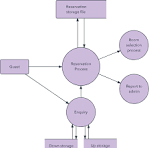
\includegraphics{Pictures/save.png}
You should follow the divide and conquer theory, so divide the overall problem into more manageable parts and develop each part or module separately. When all modules are ready, you should integrate all the modules into one system. In this phase, you should briefly describe all the modules and the functionality of these modules.
\textbf{Elements of Project Development}

\section{Data Design}
Data design will consist of how you organize, managing and manipulate the data.

\textit{Schema Design: Define the structure and explanation of schemas used in your project.}

\textit{Data Integrity and Constraints: Define and explain all the validity checks and constraints you are providing to maintain data integrity.}

\subsection{Schema Design}

\subsection{Data Integrity and Constraints}

\section{Procedural Design}
Procedural design is a systematic way for developing algorithms or procedurals.

\textit{Logic Diagrams: Define the systematical flow of procedure that improves its comprehension and helps the programmer during implementation. e.g., Control Flow Chart, Process Diagrams etc.}

\textit{Data Structures: Create and define the data structure used in your procedures.}

\textit{Algorithms Design: With proper explanations of input data, output data, logic of processes, design and explain the working of algorithms.}

\subsection{Logic Diagrams}

\subsection{Data Structures}

\subsection{Algorithms Design}

\section{User interface design}
Define user, task, environment analysis and how you intend to map those requirements in order to develop a “User Interface”. Describe the external and internal components and the architecture of your user interface. Show some rough pictorial views of the user interface and its components.

\section{Security Issues}
Discuss Real-time considerations and Security issues related to your project and explain how you intend avoiding those security problems. What are your security policy plans and architecture?

\section{Test Cases Design}
Define test cases, which will provide easy detection of errors and mistakes with in a minimum period of time and with the least effort. Explain the different conditions in which you wish to ensure the correct working of your software.